%---------------------------------------------------------------------------
% MBS Benchmark A03: Andrew's Mechanism
%---------------------------------------------------------------------------
%
% LaTeX Template: Jacobs Landscape Poster
% Created by:
% Computational Physics and Biophysics Group, Jacobs University
% https://teamwork.jacobs-university.de:8443/confluence/display/CoPandBiG/LaTeX+Poster
\documentclass[final]{beamer}

\usepackage[scale=1.24]{beamerposter} % Use the beamerposter package for laying out the poster

\usetheme{confposter} % Use the confposter theme supplied with this template

\setbeamercolor{block title}{fg=ngreen,bg=white} % Colors of the block titles
\setbeamercolor{block body}{fg=black,bg=white} % Colors of the body of blocks
\setbeamercolor{block alerted title}{fg=white,bg=dblue!70} % Colors of the highlighted block titles
\setbeamercolor{block alerted body}{fg=black,bg=dblue!10} % Colors of the body of highlighted blocks
% Many more colors are available for use in beamerthemeconfposter.sty

%-----------------------------------------------------------
% Define the column widths and overall poster size
% To set effective sepwid, onecolwid and twocolwid values, first choose how many columns you want and how much separation you want between columns
% In this template, the separation width chosen is 0.024 of the paper width and a 4-column layout
% onecolwid should therefore be (1-(# of columns+1)*sepwid)/# of columns e.g. (1-(4+1)*0.024)/4 = 0.22
% Set twocolwid to be (2*onecolwid)+sepwid = 0.464
% Set threecolwid to be (3*onecolwid)+2*sepwid = 0.708

\newlength{\sepwid}
\newlength{\onecolwid}
\newlength{\twocolwid}
\newlength{\threecolwid}
\setlength{\paperwidth}{48in} % A0 width: 46.8in
\setlength{\paperheight}{36in} % A0 height: 33.1in
\setlength{\sepwid}{0.024\paperwidth} % Separation width (white space) between columns
\setlength{\onecolwid}{0.301\paperwidth} % Width of one column
\setlength{\twocolwid}{0.602\paperwidth} % Width of two columns
\setlength{\threecolwid}{0.903\paperwidth} % Width of three columns
\setlength{\topmargin}{-0.5in} % Reduce the top margin size
%-----------------------------------------------------------

\usepackage{graphicx}  % Required for including images
\graphicspath{{../MBSfigures/}}
\usepackage{booktabs} % Top and bottom rules for tables

\usepackage{multirow}
\usepackage{siunitx}

\title{MBS Benchmark A03: Andrew's Mechanism} % Poster title


%----------------------------------------------------------------------------------------

\begin{document}

%\addtobeamertemplate{block end}{}{\vspace*{2ex}} % White space under blocks
%\addtobeamertemplate{block alerted end}{}{\vspace*{2ex}} % White space under highlighted (alert) blocks

\setlength{\belowcaptionskip}{2ex} % White space under figures
\setlength\belowdisplayshortskip{2ex} % White space under equations

\begin{frame}[t] % The whole poster is enclosed in one beamer frame

\begin{columns}[t] % The whole poster consists of three major columns, the second of which is split into two columns twice - the [t] option aligns each column's content to the top

\begin{column}{\sepwid}\end{column} % Empty spacer column

\begin{column}{\twocolwid} % The first column

%----------------------------------------------------------------------------------------
%	OBJECTIVES
%----------------------------------------------------------------------------------------

\begin{alertblock}{Benchmark Objective}
The NMS benchmark problem \textbf{A03} shows a very small time scale, thus making it difficult to simulate for solvers that cannot reach small time steps~\cite{gonzalez2006benchmarking}.
\end{alertblock}



%----------------------------------------------------------------------------------------
%    BENCHMARK DESCRIPTION
%----------------------------------------------------------------------------------------





\begin{columns}[t, totalwidth=\twocolwid]

\begin{column}{\onecolwid}
\begin{block}{Benchmark Description}
Andrew's mechanism~\cite{Schiehlen1990Multibody} (Fig.~\ref{FIG:AndrewMechanism}) is a planar system composed of seven bodies interconnected through revolution joints, and driven by a motor located in O.
Detailed information about the mechanical structure of each body is reported in  Table~\ref{TAB:PointsInGround}. Positions of reference systems are presented in Fig.~\ref{FIG:AndrewMechanismElements}

\end{block}


\begin{figure}
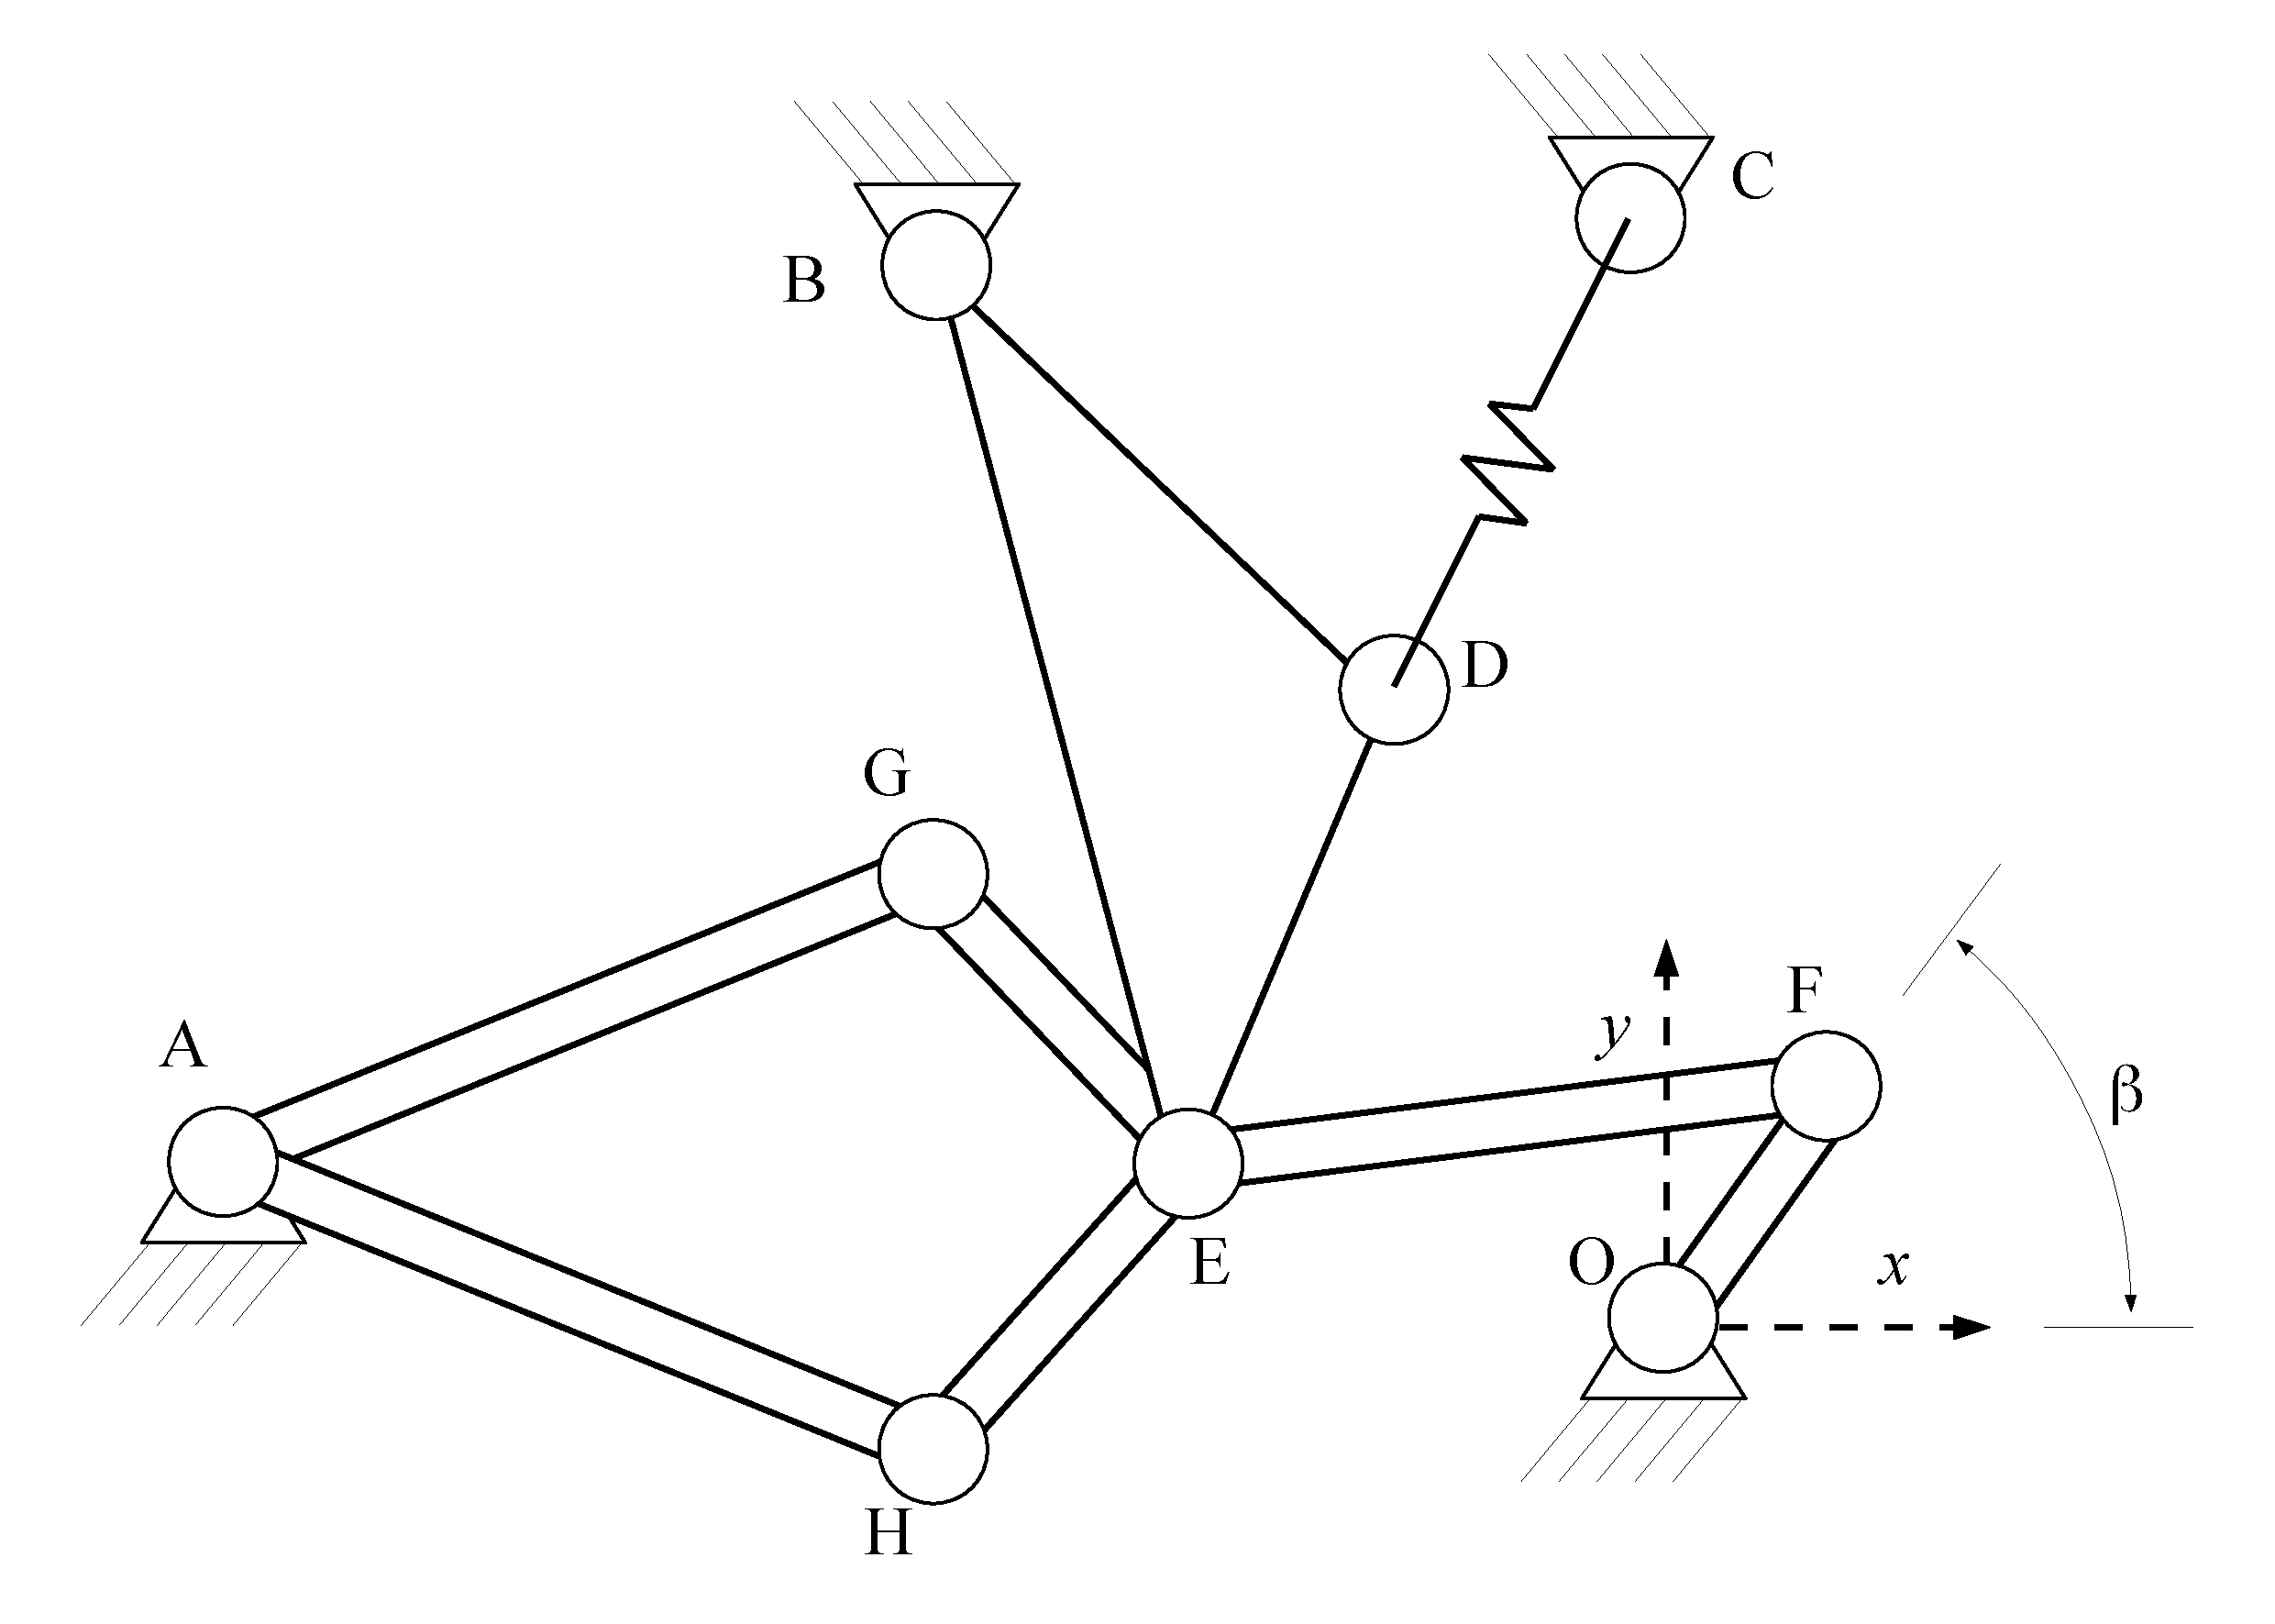
\includegraphics[width=0.8\linewidth]{3MBS_Andrew.pdf}
\caption{Andrew's mechanism sketch.}
\label{FIG:AndrewMechanism}
\end{figure}


\begin{table}
\vspace{2ex}
\begin{tabular}{ll}
\toprule
Spring coefficient & $\SI{4530}{\newton / \metre}$\\
Spring rest length & $\SI{0.07785}{\metre}$\\
Motor torque & $\SI{0.033}{\newton \per \metre}$\\
\bottomrule
\end{tabular}
 \label{TAB:SystemProperties}
\caption{System Properties and Configuration}
\end{table}



\begin{table}[h]
\centering
	\label{TAB:RodsProperties}	
	\begin{tabular}[b]{cccccc}
		\toprule
			& \multicolumn{2}{c}{Center of Mass (CoM)} & Mass & Inertia (CoM) & Length \\
			&	X [m]	&	Y [m]	&	[Kg]	&	[$Kg m^2$]	&	[m]	\\
		\midrule		
		OF	&	0.00092	&	0	&	0.04325	&	2.194$e^{-6}$	&	0.007	\\
		FE	&	-0.0115	&	0	&	0.00365	&	4.41$e^{-7}$	&	0.028	\\
		EG	&	0	&	0.01421	&	0.00706	&	5.667$e^{-7}$	&	0.02	\\
		AG	&	0.02308	&	0.00916	&	0.0705	&	1.169$e^{-5}$	&	0.04	\\
		AH	&	-0.00449	&	-0.01228	&	0.05498	&	1.912$e^{-5}$	&	0.04	\\
		HE	&	-0.01421	&	0	&	0.00706	&	5.667$e^{-7}$	&	0.02	\\
		\bottomrule
	\end{tabular}
	
	\caption{Rod Elements Properties}
\end{table}
\end{column}

\begin{column}{\onecolwid}

\begin{table}[!h]
\centering
    \label{TAB:TriangleProperties}
\begin{tabular}{ccccccc}
\toprule
\multicolumn{2}{c}{Center of Mass (CoM)}                                  & \multicolumn{1}{c}{Mass}                     & \multicolumn{1}{c}{Inertia}                        & \multicolumn{1}{|c}{Point} & \multicolumn{1}{c}{X {[}m{]}} & \multicolumn{1}{c}{Y {[}m{]}} \\ \cline{5-7} 
X {[}m{]}                & \multicolumn{1}{c}{Y {[}m{]}}                 & \multicolumn{1}{c}{{[}Kg{]}}                 & \multicolumn{1}{c}{Kg~$m^2$}                       & \multicolumn{1}{|c}{B}     & \multicolumn{1}{c}{0}         & \multicolumn{1}{c}{0}         \\ \cline{1-4}
\multirow{2}{*}{0.01043} & \multicolumn{1}{c}{\multirow{2}{*}{-0.01874}} & \multicolumn{1}{c}{\multirow{2}{*}{0.02373}} & \multicolumn{1}{c}{\multirow{2}{*}{5.255$e^{-6}$}} & \multicolumn{1}{|c}{D}     & \multicolumn{1}{c}{0.02}      & \multicolumn{1}{c}{-0.018}    \\
                         & \multicolumn{1}{c}{}                          & \multicolumn{1}{c}{}                         & \multicolumn{1}{c}{}                               & \multicolumn{1}{|c}{E}     & \multicolumn{1}{c}{0}         & \multicolumn{1}{c}{-0.035}    \\
                         
\bottomrule
\end{tabular}
\caption{Triangular Element Properties, points defined in $X_{BDE}$-$Y_{BDE}$ SoR}
\end{table}


\begin{figure}[h]
\centering
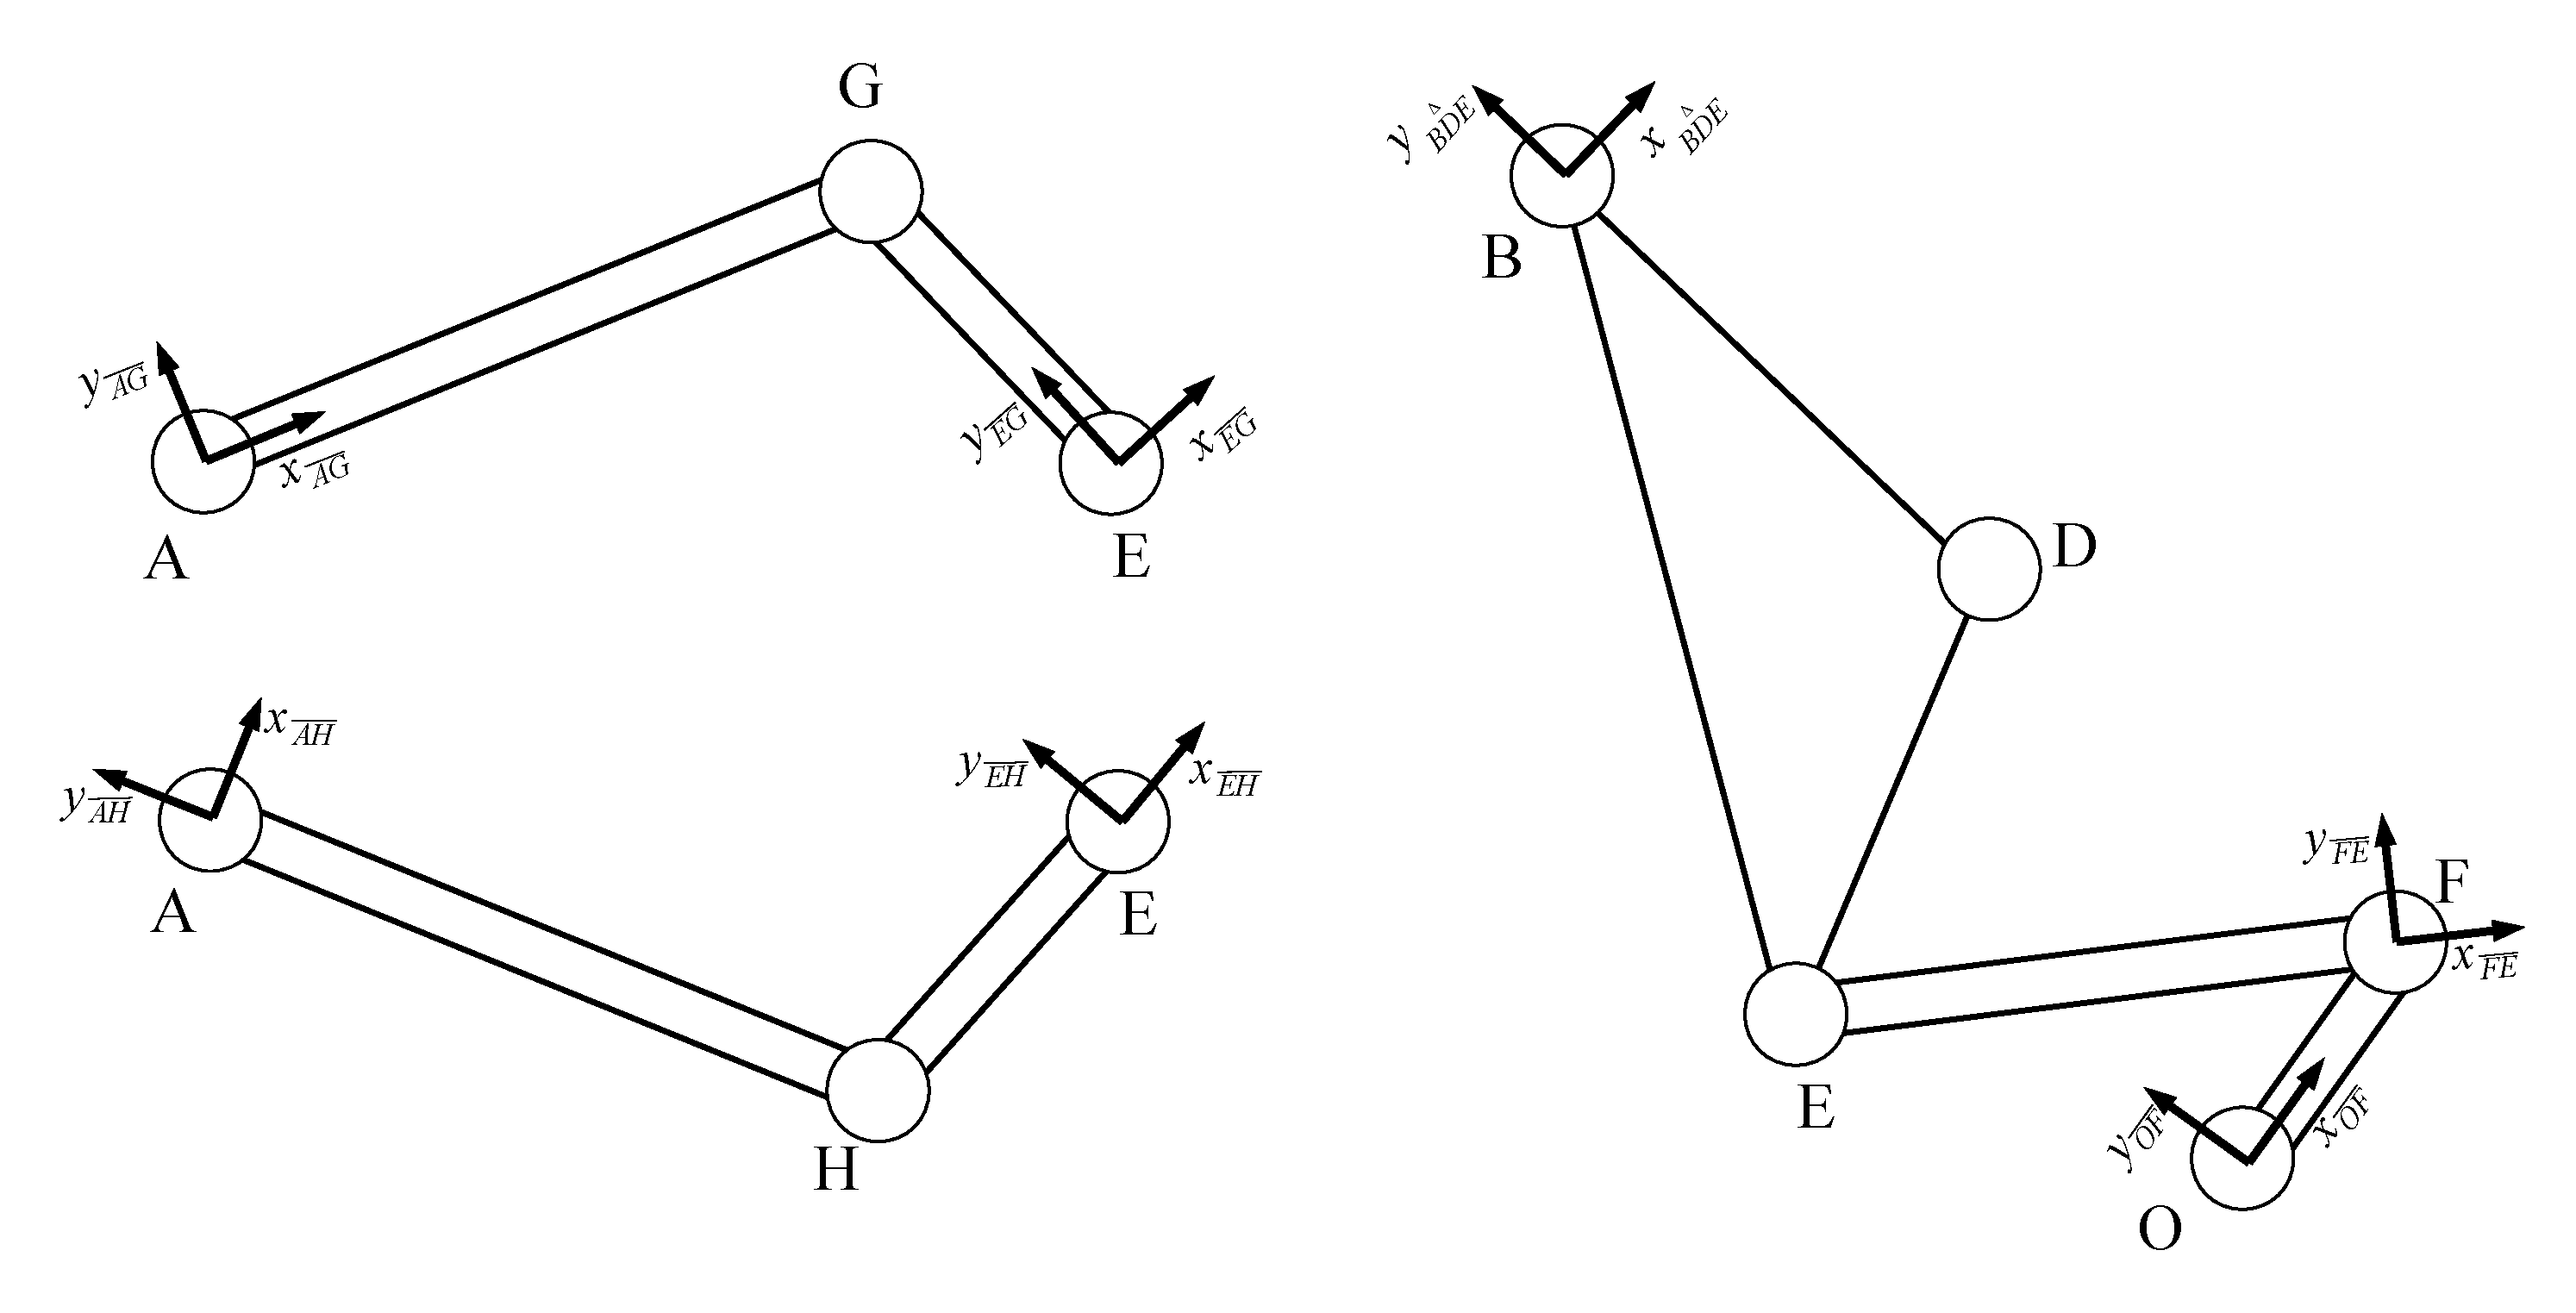
\includegraphics[width=0.8\textwidth]{3MBS_Andrew_OABCDEFG.pdf}
\caption{Systems of Reference defined for each body of the mechanism.}
\label{FIG:AndrewMechanismElements}
\end{figure}

\begin{columns}[t,totalwidth=\onecolwid]

%--------------------------

\begin{column}{7.2in}
\begin{table}[h]
\begin{tabular}{ccc}
\toprule
Point & X {[}m{]} & Y{[}m{]} \\ 
\midrule
O     & 0         & 0        \\
A     & -0.06934  & -0.00227 \\
B     & 0.03635   & 0.03273  \\
C     & 0.014     & 0.072\\
\bottomrule
\end{tabular}

\caption{Points in ground $X$-$Y$ SoR}
\label{TAB:PointsInGround}
\end{table}
\end{column}


\begin{column}{7.2in}
\begin{table}[h]
\begin{tabular}{cc}
\toprule
 & Angle [rad] \\ 
\midrule
$\beta$     &-0.0620        \\
$\hat{OFE}$     &0        \\
$\hat{FEB}$     &2.088        \\
$\hat{FEG}$     &2.341        \\
$\hat{EGA}$     &1.792        \\
$\hat{EHA}$     &1.348        \\
\bottomrule
\end{tabular}

\caption{Initial Joints Position}
\label{TAB:InitialAngles}
\end{table}
\end{column}

\end{columns}



%----------------------------------------------------------------------------------------
%	CONTACT INFORMATION
%----------------------------------------------------------------------------------------


\setbeamercolor{block alerted title}{fg=black,bg=norange} % Change the alert block title colors
\setbeamercolor{block alerted body}{fg=black,bg=white} % Change the alert block body colors

\begin{alertblock}{Contact Information}
Rehabilitation Engineering Group\\Department of Management and Engineering\\ University of Padua

\begin{itemize}
\item Web: \href{http://reg.gest.unipd.it}{http://reg.gest.unipd.it}
\item Email: \href{mailto:reg.info@gest.unipd.it}{reg.info@gest.unipd.it}
\end{itemize}
 
\end{alertblock}

\end{column}
  

\end{columns}


\end{column}
\begin{column}{\onecolwid} % The third column


%----------------------------------------------------------------------------------------
%    RESULTS
%----------------------------------------------------------------------------------------

\begin{block}{Results}
The dynamic simulation of the \textbf{A03} benchmark was executed for \SI{0.5}{\second}.
The starting position of the simulation is defined by the values in Tab.~\ref{TAB:InitialAngles}. 
The objective of the simulation is to measure $F$ displacements and compare them with the reference solution~\cite{gonzalez2006benchmarking}.

The simulation with OpenSim perfectly match the reference values as shown in Fig.~\ref{FIG:simulationPlot} for a \SI{0.05}{\second} simulation. 


\begin{figure}[h]
\centering
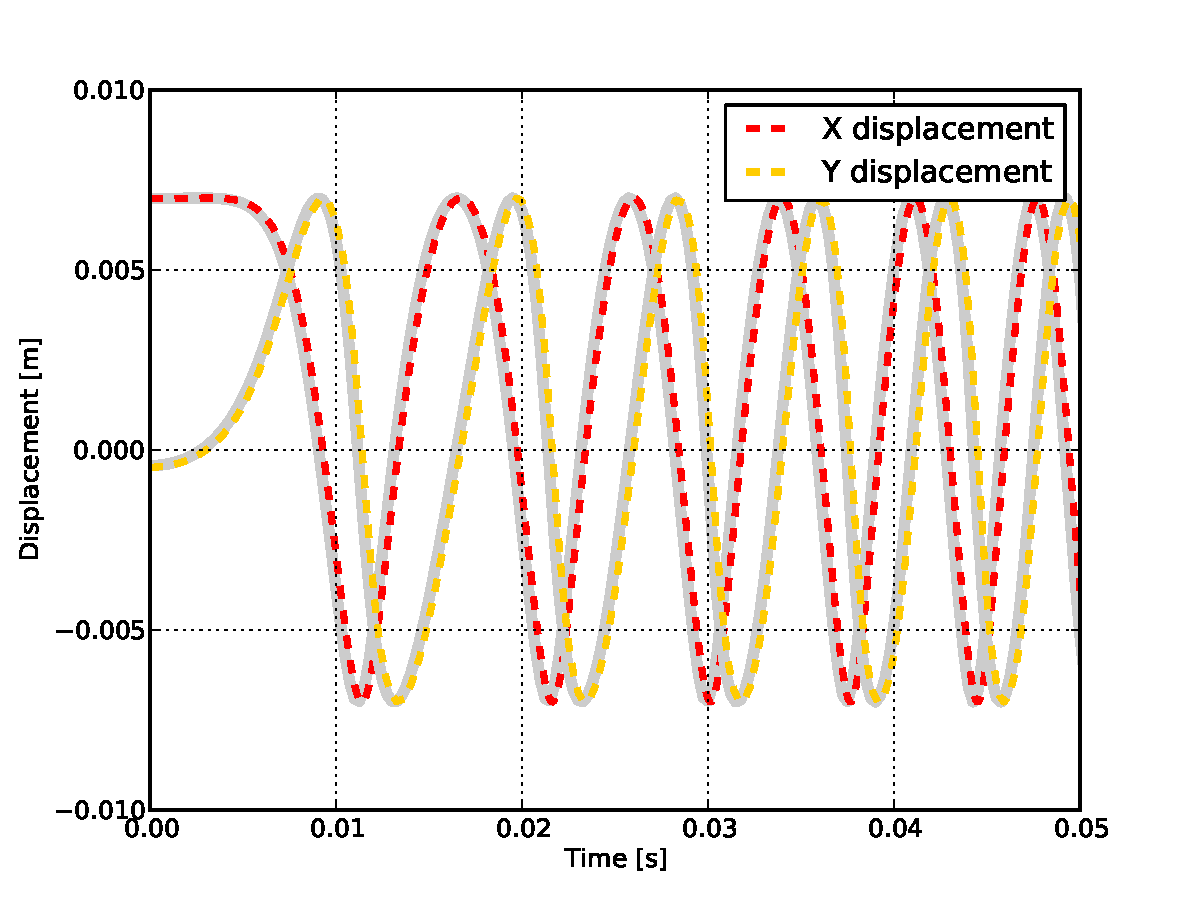
\includegraphics[width=0.8\textwidth]{3MBS_PlotResults.pdf}
\caption{Comparison of the point $F$ displacements between Andrew's mechanism model simulated in OpenSim
(dashed lines) and MBS benchmark reference (grey lines).}
\label{FIG:simulationPlot}
\end{figure}

\end{block}

\begin{block}{Download}
\begin{itemize}
\item MBS Benchamark available at: \url{http://goo.gl/ySQ5me}
\item OpenSim implementation available at: \url{http://goo.gl/R9tl3z}
\item Videos of OpenSim simulation available at: \url{http://goo.gl/9BBdZH}
\end{itemize}
\end{block}
%----------------------------------------------------------------------------------------
%	REFERENCES
%----------------------------------------------------------------------------------------

\begin{block}{References}

\begin{thebibliography}{99}

\bibitem{gonzalez2006benchmarking} M. Gonz{\'a}lez, D. Dopico, U. Lugr{\'\i}s, J. Cuadrado, \textit{``A benchmarking system for MBS simulation software: Problem standardization and performance measurement,''} 	in Multibody System Dyn., vol. 6, no.2,  2006, pp. 179--190.

\bibitem{Schiehlen1990Multibody} M. Schiehlen, \textit{Multibody Systems Handbook}. Springer-Verlag, Dordrecht (1990)

\end{thebibliography}

\end{block}



%----------------------------------------------------------------------------------------

\end{column} % End of the third column

\end{columns} % End of all the columns in the poster

\end{frame} % End of the enclosing frame

\end{document}
